Para esta etapa del proyecto se detectarán los bad smells del código existente del pro proyecto y se aplicarán técnicas de refactoring e ingeniería para resolverlos.

\section{Revisión de los Shared Layout de las vistas}
\subsection{Librerías de terceros innecesarias}
\begin{itemize}
	\item \textbf{Síntoma:} Existen librerías de terceros procedentes de la plantilla que no se utilizan en ningún momento.
	\item \textbf{Solución:} Revisar que librerías se están usando dentro del proyecto. 
	\item \textbf{Procedimiento:} Se eliminó la carpeta que contenía los elementos de la plantilla, se migraron los paquetes a bower y se reciclo las hojas de estilos. Además, se escribió comentarios indicando la función que cumple cada uno.
\end{itemize}

\begin{lstlisting}[language=html]
@* CSS *@
<!-- Fuentes -->
<!-- Plugins -->
<!-- Bootstrap -->
<link href="~/lib/bootstrap/dist/css/bootstrap.css" rel="stylesheet" /> 
 <!-- Mensajes emergentes -->
<link href="~/lib/toastr/toastr.css" rel="stylesheet" />
<!-- Iconos -->
<!-- Iconos principales -->
<link href="~/lib/fontawesome/css/font-awesome.css" rel="stylesheet" /> 
<!-- Estilos de la aplicacion -->
<!-- Normalizacion de elementos -->
<link href="~/css/components.css" rel="stylesheet" /> 

@* JavaScript *@
<!-- jQuery -->
<script src="~/lib/jquery/dist/jquery.min.js"></script> 
<!-- Bootstrap -->
<script src="~/lib/bootstrap/dist/js/bootstrap.min.js"></script> 
<!-- Waypoints: Trigger para iniciar funcion -->
<script src="~/lib/waypoints/lib/jquery.waypoints.min.js"></script> 
\end{lstlisting}

\subsection{Error en la carga de las vistas}
\begin{itemize}
	\item \textbf{Síntoma:} Las vistas de la aplicación presentan un ligero retardo al cargar la data.
	\item \textbf{Solución:} Revisar las directivas de Angular. 
	\item \textbf{Procedimiento:} Se agregó la directiva ng-cloak
\end{itemize}

\begin{lstlisting}[language=html]
<div class="row" ng-app="app" ng-controller="alumnosController as vm">
	<wait-cursor display-when="vm.isBusy"></wait-cursor>
	<!-- Tabla de visualizacion -->
	<div ... ng-cloak>
		...
	</div>
</div>
\end{lstlisting}

\subsection{Error en la carga de las vistas}
\begin{itemize}
	\item \textbf{Síntoma:} Los archivos javascript de la aplicación están mezclados con los controladores angular.
	\item \textbf{Solución:} Colocar todos los controladores dentro de una carpeta.
	\item \textbf{Procedimiento:} Se creó la carpeta ``angular" para trasladar los controladores y se cambió la ruta de los paquetes en las vistas.
\end{itemize}

\begin{figure}[h]
	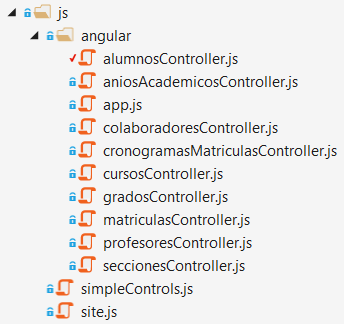
\includegraphics[width=0.5\textwidth]{1.png}
	\centering
\end{figure}

\begin{lstlisting}[language=html]
@section scripts {
	...
	<script src="~/js/angular/app.js"></script>
	<script src="~/js/angular/alumnosController.js"></script>
	...
}
\end{lstlisting}

\subsection{Validación de los nested objects}
\begin{itemize}
	\item \textbf{Síntoma:} El controlador no valida los nested objects y se valida los objetos manualmente.
	\item \textbf{Bad Smell:} Duplicated code.
	\item \textbf{Solución:} Crear una clase que realice este proceso iterativamente.
	\item \textbf{Procedimiento:} Se creó dos clases, una llamada ``CompositeValidationResult" y la otra ``ValidateObjectAttribute" que agregan un atributo a los decoradores de validación del modelo para que puedan usarse en todos los DTO.
\end{itemize}

\begin{figure}[h]
	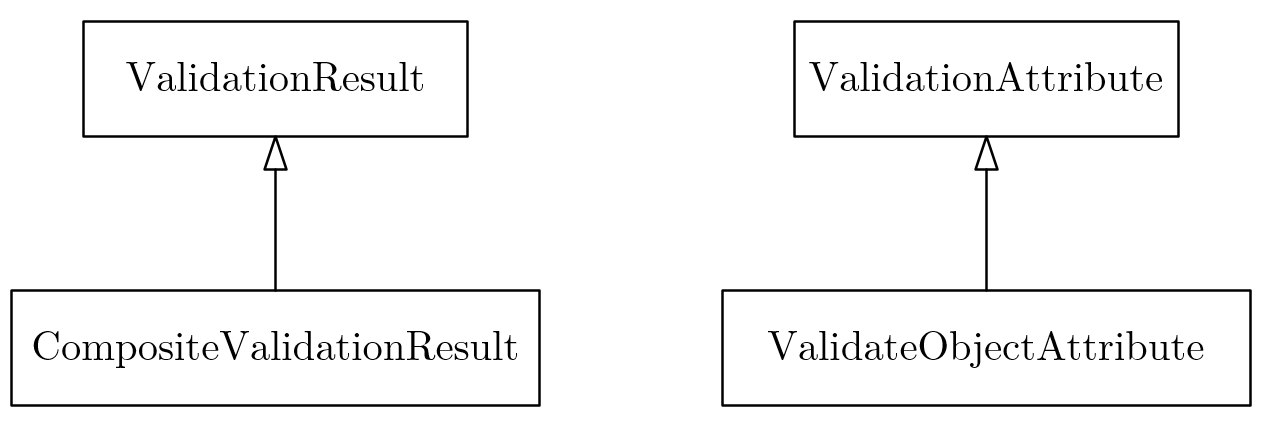
\includegraphics[width=0.7\textwidth]{2.png}
	\centering
\end{figure}

\begin{lstlisting}[language={[Sharp]C}]
public class AlumnoViewModel
{
	...
	[Required, ValidateObject]
	public virtual ApoderadoViewModel Apoderado { get; set; }
	...
}
\end{lstlisting}

\subsection{Duplicidad en el mapeo}
\begin{itemize}
	\item \textbf{Síntoma:} Se está mapeando el objeto dos veces, una para validar algún atributo y otro para transaccionar.
	\item \textbf{Bad Smell:} Duplicated code.
\end{itemize}

\begin{lstlisting}[language={[Sharp]C}]
public class AlumnoViewModel
[HttpPost()]
public async Task<IActionResult> PostAlumno([FromBody] AlumnoViewModel alumnoDetails)
{
	...
	if (!_repository.IsDniValido(Mapper.Map<Alumno>(alumnoDetails)))
		ModelState.AddModelError("otros", "Este DNI ya fue registrado.");

	if (ModelState.IsValid)
	{
		var _newAlumno = Mapper.Map<Alumno>(alumnoDetails);
		...
	}
	...
}
\end{lstlisting}

\begin{itemize}	
	\item \textbf{Solución:} Extraer las sentencias duplicadas y colocarlo en una variable.
	\item \textbf{Técnica:} Extract variable.
\end{itemize}
	
\begin{lstlisting}[language={[Sharp]C}]
[HttpPost()]
public async Task<IActionResult> PostAlumno([FromBody] AlumnoViewModel alumnoDetails)
{
	...
	var alumno = Mapper.Map<Alumno>(alumnoDetails);

	if (!_repository.IsDniValido(alumno))
		ModelState.AddModelError("otros", "Este DNI ya fue registrado.");

	if (ModelState.IsValid)
	{
		_repository.AddAlumno(alumno);
		...
	}
	...
}
\end{lstlisting}
	
\subsection{Ruta de los controlador API}
\begin{itemize}
	\item \textbf{Síntoma:} Se está repitiendo en cada acción la ruta del controlador.
	\item \textbf{Bad Smell:} Duplicated code.
\end{itemize}

\begin{lstlisting}[language={[Sharp]C}]
public class AlumnosController : Controller
{
	...	
	
	[HttpGet("api/alumnos"))]
	public IActionResult GetAllAlumnos()
	{ ... }
	
	[HttpGet("api/alumnos/{id}")]
	public IActionResult GetAlumno(int id)
	{ ... }
	
	...
}
\end{lstlisting}

\begin{itemize}	
	\item \textbf{Solución:} Utilizar el decorador Route para indicar la ruta del controlador. También indicar la versión del API y cambiar el nombre de las acciones según convenciones.
\end{itemize}

\begin{lstlisting}[language={[Sharp]C}]
[Route("api/v2/[controller]")]
public class AlumnosController : Controller
{
	...	
	
	[HttpGet()]
	public IActionResult GetAllAlumnos()
	{ ... }
	
	[HttpGet("{id}")]
	public IActionResult GetAlumno(int id)
	{ ... }
	
	...
}
\end{lstlisting}

%%%%%%%%%%%%%%%%%%%%%%%%%%%%%%%%%%%%%%%%%%%%%

\subsection{Sobrecarga de Entity Framework}
\begin{itemize}
	\item \textbf{Síntoma:} Se está accediendo muchas veces a un atributo del objeto
\end{itemize}

\begin{lstlisting}[language={[Sharp]C}]
public void ToggleEstado(int id)
{
	var colaborador = Get(id);
	_context.Colaboradores.Attach(colaborador).State = EntityState.Modified;
	
	if (colaborador.Estado == "1")
		colaborador.Estado = "3";
	else if (colaborador.Estado == "3")
		colaborador.Estado = "1";
	
	_context.Update(colaborador);
}
\end{lstlisting}

\begin{itemize}	
	\item \textbf{Técnica:} Extract variable.
	\item \textbf{Solución:} Extraer la operación en una variable temporal.
\end{itemize}

\begin{lstlisting}[language={[Sharp]C}]
public void ToggleEstado(int id)
{
	var colaborador = Get(id);
	_context.Colaboradores.Attach(colaborador).State = EntityState.Modified;
	
	var estado = colaborador.Estado;
	
	colaborador.Estado = estado == "1" ?  "3" : estado == "3" ? "1" : estado;
}
\end{lstlisting}

%%%%%%%%%%%%%%%%%%%%%%%%%%%%%%%%%%%%%%%%%%%%%

\subsection{Actualización de campos}
\begin{itemize}
	\item \textbf{Síntoma:} Se está pasando cada uno de los atributos para la actualización del objeto.
\end{itemize}

\begin{lstlisting}[language={[Sharp]C}]
public void UpdateAlumno(Alumno entity)
{
	var thisAlumno = GetAlumnoById(entity.Id);
	thisAlumno.ApellidoPaterno = alumnoToUpdate.ApellidoPaterno;
	thisAlumno.ApellidoMaterno = alumnoToUpdate.ApellidoMaterno;
	thisAlumno.Nombres = alumnoToUpdate.Nombres;
	thisAlumno.Dni = alumnoToUpdate.Dni;
	thisAlumno.Sexo = alumnoToUpdate.Sexo;
	thisAlumno.Direccion = alumnoToUpdate.Direccion;
	thisAlumno.FechaNacimiento = alumnoToUpdate.FechaNacimiento;
	
	_context.Update(thisAlumno);
}
\end{lstlisting}

\begin{itemize}
	\item \textbf{Solución:} Utilizar Entries de Entity Framework para determinar los comportamientos de las entidades y no alterar los Nested Objects.
\end{itemize}

\begin{lstlisting}[language={[Sharp]C}]
public Alumno UpdateAlumno(Alumno entity)
{
	_context.Entry(entity).State = EntityState.Modified;
}
\end{lstlisting}

%%%%%%%%%%%%%%%%%%%%%%%%%%%%%%%%%%%%%%%%%%%%%

\subsection{Método SearchCursos en controlador de cursos}
\begin{itemize}
	\item \textbf{Síntoma:} El método SearchCursos se encarga de listar los cursos que dicta un profesor está en un controlador que no le corresponde.
	\item \textbf{Bad Smell:} Intimidad inadecuada.
\end{itemize}

\begin{lstlisting}[language={[Sharp]C}]
public class CursosController : Controller
{
	...	
	[HttpGet("{id}")]
	public IActionResult GetCursosDisponibles(int id)
	{
		try
		{
			_logger.LogInformation("Recuperando la lista de cursos que dicta el profesor.");
			var results = _repository.GetCursosByIdProfesor(id);
			return Ok(Mapper.Map<IEnumerable<CursoViewModel>>(results));
		}
		catch (Exception ex)
		{
			_logger.LogError($"No se pudo recuperar los cursos: {ex}");
			return BadRequest("No se pudo recuperar la información.");
		}
	}	
	...
}
\end{lstlisting}

\begin{itemize}
	\item \textbf{Técnica:} Move Method.
	\item \textbf{Solución:} Trasladar este método al controlador de profesores para implementar el API Rest correctamente. 
\end{itemize}

\begin{lstlisting}[language={[Sharp]C}]
public class ProfesoresController : Controller
{
	...
	[HttpGet("{id}")]
	public IActionResult GetCursosDisponibles(int id)
	{
		try
		{
			_logger.LogInformation("Recuperando la lista de cursos que dicta el profesor.");
			var results = _repository.GetCursosByIdProfesor(id);
			return Ok(Mapper.Map<IEnumerable<CursoViewModel>>(results));
		}
		catch (Exception ex)
		{
			_logger.LogError($"No se pudo recuperar los cursos: {ex}");
			return BadRequest("No se pudo recuperar la información.");
		}
	}	
	...
}
\end{lstlisting}

%%%%%%%%%%%%%%%%%%%%%%%%%%%%%%%%%%%%%%%%%%%%%

\subsection{Lógica de negocio en el controlador}
\begin{itemize}
	\item \textbf{Síntoma:} El controlador tiene código de la lógica del negocio; las tareas que deberían ejecutarse en el repositorio.
	\item \textbf{Bad Smell:} Intimidad inadecuada.
\end{itemize}

\begin{lstlisting}[language={[Sharp]C}]
public async Task<IActionResult> PostUpdateProfesorCurso([FromBody] CursoProfesorViewModel profesorDetails)
{
	...
	if (ModelState.IsValid)
	{
		var profesor = Mapper.Map<Profesor>(profesorDetails.Profesor);
		var curso = Mapper.Map<Curso>(profesorDetails.Curso);
		...
	}
	...
}
\end{lstlisting}

\begin{itemize}
	\item \textbf{Técnica:} Move Method y Extract Method.
	\item \textbf{Solución:} Trasladar el código al repositorio creando un método que realice las tareas de mapeo.
\end{itemize}

\begin{lstlisting}[language={[Sharp]C}]
public void AssignProfesor(int id, int idProfesor)
{
	var anioAcademico = new AniosAcademicosRepository(_context).GetAnioAcademico(DateTime.Now.Year);

	if (anioAcademico != null)
	{
		var cursoAnioAcademico = _context.CursosAnioAcademico
			.Where(t => t.AnioAcademicoId == anioAcademico.Id)
			.Where(t => t.CursoId == id)
			.FirstOrDefault();	
		...
	}
}
\end{lstlisting}

%%%%%%%%%%%%%%%%%%%%%%%%%%%%%%%%%%%%%%%%%%%%%

\subsection{Uso inadecuado de procedimientos almacenados}
\begin{itemize}
	\item \textbf{Síntoma:} El método llama a un procedimiento en la base de datos.
\end{itemize}

\begin{lstlisting}[language={[Sharp]C}]
public void Update(Profesor entity)
{
	...
	_context.Database.ExecuteSqlCommand(String.Format("EXEC SP_DeleteCursos @idProfesor='{0}'", profesor.Id));
	foreach (Curso curso in cursos)
	{
    	_context.Database.ExecuteSqlCommand(
    		String.Format("EXEC SP_AddProfesorCurso @idProfesor='{0}', @idCurso='{1}'", 
    			profesor.Id, curso.Id));
	}
	...
}
\end{lstlisting}

\begin{itemize}
	\item \textbf{Técnica:} Extract Method.
	\item \textbf{Solución:} Remplazar el procedimiento almacenado con sentencias LINQ, y extraer el segmento de código que elimina los cursos actuales del profesor en un nuevo método.
\end{itemize}

\begin{lstlisting}[language={[Sharp]C}]
public void EliminarCursos(int id)
{
	var cursos = _context.ProfesorCursos
		.Where(t => t.ProfesorId == id)
		.ToList();
	
	_context.ProfesorCursos.RemoveRange(cursos);
	_context.SaveChanges();
}
\end{lstlisting}

%%%%%%%%%%%%%%%%%%%%%%%%%%%%%%%%%%%%%%%%%%%%%
\break
\subsection{Lógica de negocio en el controlador}
\begin{itemize}
	\item \textbf{Síntoma:} El controlador tiene código de la lógica del negocio; las tareas que deberían ejecutarse en el repositorio.
	\item \textbf{Bad Smell:} Intimidad inadecuada.
\end{itemize}

\begin{lstlisting}[language={[Sharp]C}]
public async Task<IActionResult> PostUpdateProfesorCurso([FromBody] CursoProfesorViewModel profesorDetails)
{
	...
	if (ModelState.IsValid)
	{
		var profesor = Mapper.Map<Profesor>(profesorDetails.Profesor);
		var curso = Mapper.Map<Curso>(profesorDetails.Curso);
		...
	}
	...
}
\end{lstlisting}

\begin{itemize}
	\item \textbf{Técnica:} Move Method y Extract Method.
	\item \textbf{Solución:} Trasladar el código al repositorio creando un método que realice las tareas de mapeo.
\end{itemize}

\begin{lstlisting}[language={[Sharp]C}]
public void AssignProfesor(int id, int idProfesor)
{
	var anioAcademico = new AniosAcademicosRepository(_context).GetAnioAcademico(DateTime.Now.Year);

	if (anioAcademico != null)
	{
		var cursoAnioAcademico = _context.CursosAnioAcademico
		.Where(t => t.AnioAcademicoId == anioAcademico.Id)
		.Where(t => t.CursoId == id)
		.FirstOrDefault();	
		...
	}
}
\end{lstlisting}

%%%%%%%%%%%%%%%%%%%%%%%%%%%%%%%%%%%%%%%%%%%%%

\subsection{Atributos que no se usan}
\begin{itemize}
	\item \textbf{Síntoma:} La clase Cursos tiene atributos que no usa.
\end{itemize}

\begin{lstlisting}[language={[Sharp]C}]
public class Curso
{      
	...
	public virtual IEnumerable<Profesor> Profesores { get; set; }	
	public virtual ICollection<ProfesorCurso> ProfesorCurso { get; set; }
	...
}

\end{lstlisting}

\begin{itemize}
	\item \textbf{Solución:} Eliminar los atributos que no usa en el modelo.
\end{itemize}

%%%%%%%%%%%%%%%%%%%%%%%%%%%%%%%%%%%%%%%%%%%%%

\subsection{Cambiar la definición de la clase CronogramaMatricula}
\begin{itemize}
	\item \textbf{Síntoma:} La clase CronogramaMatricula que era el modelo de los cronogramas de matrículas; ahora, se utilizará para cualquier tipo de cronograma dentro de un año académico. Además se usando un atributo "Nombre" como Primary Key.
\end{itemize}

\begin{lstlisting}[language={[Sharp]C}]
public class CronogramaMatricula
{
	[Key]
	[ForeignKey("AnioAcademico")]
	public int AnioAcademicoId { get; set; }
	
	[Key]
	[StringLength(30)]
	public string Nombre { get; set; }
	
	...
}
\end{lstlisting}

\begin{itemize}
	\item \textbf{Solución:} Renombrar la clase CronogramaMatricula a Cronograma. Agregar un Atributo Id para establecerlo como Primary Key.
\end{itemize}
\begin{lstlisting}[language={[Sharp]C}]
public class Cronograma
{
	[Key]
	public int Id { get; set; }

	[ForeignKey("AnioAcademico")]
	public int AnioAcademicoId { get; set; }
	
	[StringLength(30)]
	public string Nombre { get; set; }
	
	...
}
\end{lstlisting}